\section{Experiments}
\label{sec:experiments}

We evaluate three training conditions on ALFWorld's 47 unseen test tasks \cite{shridhar2021alfworld}: \textbf{Vanilla} (4{,}358 clean demonstrations), \textbf{TaxEI} (4{,}358 clean + 4{,}671 taxonomy-tagged error trajectories = 9{,}029), and \textbf{Random} (4{,}358 clean + 4{,}671 generic-labeled errors = 9{,}029). Training details are in \S\ref{sec:training_setup}. We report results across three seeds (42, 0, 123).

\subsection{Main Results}
\label{sec:main_results}

Table~\ref{tab:main_results} shows three-seed evaluation results. TaxEI degrades directionally ($-8.6$pp vs.\ Vanilla), but the difference is not statistically significant (permutation test, $p{=}0.054$, $N{=}10{,}000$). No TaxEI seed exceeds the Vanilla mean. Random injection shows minimal degradation ($-2.2$pp, $p{>}0.3$). The TaxEI--Random gap is driven by two of six task types (\texttt{pick\_cool}: $-19.0$pp; \texttt{pick\_two\_obj}: $-14.3$pp).

\begin{table}[t]
\centering
\small
\begin{tabular}{lccccc}
\toprule
\textbf{Method} & \textbf{$N$} & \textbf{s42} & \textbf{s0} & \textbf{s123} & \textbf{Mean$\pm$SD} \\
\midrule
Vanilla & 4{,}358 & 61.7 & 68.1 & 66.0 & 65.3$\pm$3.3 \\
TaxEI   & 9{,}029 & 61.7 & 46.8 & 61.7 & 56.7$\pm$8.6 \\
Random  & 9{,}029 & 66.0 & 55.3 & 68.1 & 63.1$\pm$7.0 \\
\bottomrule
\end{tabular}
\caption{Three-seed clean evaluation on ALFWorld (47 tasks, accuracy \%). TaxEI vs.\ Vanilla: $p{=}0.054$; TaxEI vs.\ Random: $p{=}0.170$; Random vs.\ Vanilla: $p{>}0.3$ (pooled permutation, 10K). Note: TaxEI/Random use 9{,}029 samples ($2.1\times$ vanilla). The dose-response ablation (Table~\ref{tab:dose_response}) controls for data volume at a fixed 4{,}358 total.}
\label{tab:main_results}
\end{table}

At full training scale, standard deviations follow Vanilla (3.3pp) $<$ Random (7.0pp) $<$ TaxEI (8.6pp), though not statistically confirmed at $n{=}3$. The dose-response ablation (\S\ref{sec:dose_response}) reveals this variance is dose-dependent: deterministic at 25\% (SD${=}$1.2pp) but chaotic at 50\% (SD${\approx}$12pp).

\subsection{Dose-Response}
\label{sec:dose_response}

To control for data volume, we fix total training size at 4{,}358 and vary the injection ratio (Table~\ref{tab:dose_response}, Figure~\ref{fig:dose_response}). Multi-seed results at 25\% and 50\% reveal a dual regime.

\begin{table}[t]
\centering
\small
\begin{tabular}{lccccc}
\toprule
\textbf{Dose} & \textbf{s42} & \textbf{s0} & \textbf{s123} & \textbf{Mean$\pm$SD} & \textbf{$\Delta$} \\
\midrule
\multicolumn{6}{l}{\textit{TaxEI}} \\
10\%$^\dagger$ & 61.7 & --- & --- & 61.7 & --- \\
25\%  & 48.9 & 46.8 & 46.8 & 47.5$\pm$1.2 & $-$17.8 \\
50\%  & 51.1 & 70.2 & 46.8 & 56.0$\pm$12.4 & $-$9.3 \\
\midrule
\multicolumn{6}{l}{\textit{Random}} \\
10\%$^\dagger$ & 68.1 & --- & --- & 68.1 & --- \\
25\%  & 55.3 & 61.7 & 51.1 & 56.0$\pm$5.3 & $-$9.3 \\
50\%  & 57.4 & 46.8 & 70.2 & 58.1$\pm$11.7 & $-$7.2 \\
\bottomrule
\end{tabular}
\caption{Dose-response ablation (fixed 4{,}358 total). $\Delta$: mean change vs.\ vanilla (65.3$\pm$3.3). $^\dagger$Single seed (seed=42); $\Delta$ omitted as baseline differs from the 3-seed mean used for other rows. At 25\%, TaxEI degrades deterministically (SD${=}$1.2pp). At 50\%, variance explodes (SD${\approx}$12pp), with seeds spanning 46.8--70.2\%.}
\label{tab:dose_response}
\end{table}

\begin{figure}[t]
\centering
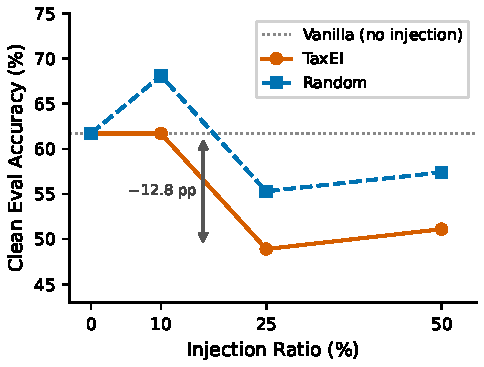
\includegraphics[width=\columnwidth]{figures/paper/fig1_dose_response.pdf}
\caption{Dose-response (seed=42 only). 3-seed data in Table~\ref{tab:dose_response} reveals non-monotonic dose-response with regime bifurcation at 25\%$\to$50\%.}
\label{fig:dose_response}
\end{figure}

At 25\%, TaxEI degrades deterministically: all three seeds converge to $\sim$47\% ($-17.8$pp, SD${=}$1.2pp). Random also degrades ($-9.3$pp, SD${=}$5.3pp). At 50\%, both methods exhibit extreme seed sensitivity (SD${\approx}$12pp), with seeds ranging from 46.8\% to 70.2\%---the latter exceeding all vanilla seeds. The dose-response is non-monotonic: 50\% TaxEI mean (56.0\%) exceeds 25\% mean (47.5\%). At 10\% (single seed), TaxEI matches Vanilla exactly; Random achieves 68.1\%, within vanilla seed range.

\subsection{Recovery Evaluation}
\label{sec:recovery}

We test whether error-trained models recover from injected errors at inference time (round-robin operator injection, 47 tasks, seed=42 only, preliminary). TaxEI achieves 59.6\% recovery (vs.\ Vanilla 61.7\%, Random 63.8\%)---no statistically significant improvement. The uniform 0\% detection rate (seed=42) suggests taxonomy labels were not internalized during SFT---models learned trajectory patterns rather than error classification.

\subsection{Per-Operator Local/Global Split}
\label{sec:operator_split}

Figure~\ref{fig:operator_gradient} decomposes recovery by operator (seed=42, $N{=}11$--$12$). Local operators (C4 observation masking: 7/11 vs.\ 6/11, $+9.1$pp; P1 step swap: 7/12 vs.\ 7/12, $0.0$pp) are neutral-to-beneficial; global operators (C1 context truncation: 8/12 vs.\ 9/12, $-8.3$pp; P2 sub-goal deletion: 6/12 vs.\ 7/12, $-8.3$pp) are harmful. Local errors leave the causal structure intact; global errors propagate downstream. These results are exploratory ($N{=}11$--$12$).

\begin{figure}[t]
\centering
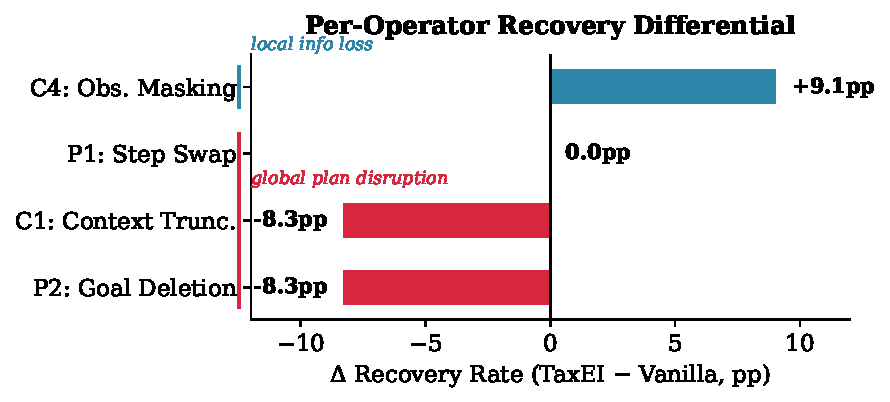
\includegraphics[width=\columnwidth]{figures/paper/fig2_operator_gradient.pdf}
\caption{Per-operator recovery delta (TaxEI $-$ Vanilla, seed=42). $N{=}11$--$12$; $\pm1$ task $\approx$ $\pm$8--9pp. Exploratory.}
\label{fig:operator_gradient}
\end{figure}

\subsection{Training-Evaluation Paradox}
\label{sec:paradox}

At $\geq$25\% injection, models can achieve \emph{lower} training loss but \emph{worse} evaluation performance. For seed=42, TaxEI-50\% reaches final loss 0.259 (vs.\ Vanilla 0.288) yet evaluates at 51.1\% (vs.\ 61.7\%). This paradox does not hold at 10\%, where training loss (0.308) remains above Vanilla. Two explanations are plausible: memorization of noise \cite{arpit2017memorization,zhou2023lima} and distribution shift at high injection ratios. The extreme seed variance at 50\% suggests this paradox is seed-dependent: TaxEI-50\% seed=0 achieves 70.2\% despite similar training dynamics.

